\section{Conformance and Reproducibility}
\label{sec:conformance}

Agent Manifest is realized by an open-source Python SDK (\texttt{agent-manifest}) and
a formal conformance suite. The SDK provides the data model, signing
(\texttt{generate\_ed25519}, signers/verifiers), verification
(\texttt{verify\_manifest}), canonicalization, Merkle construction, delegation and
revocation, hardware-attestation providers (TPM, SEV-SNP, TDX, OPAQUE) with
auto-selection, and a \texttt{manifest} CLI (\texttt{keygen}, \texttt{create},
\texttt{sign}, \texttt{attest}, \texttt{verify}, \texttt{revoke}).

\subsection{Conformance levels}

Conformance is defined at four assurance levels, each adding evidence
(Table~\ref{tab:levels}). A claim of conformance is checked, not asserted. The suite
runs against versioned example manifests: software-only, TPM-attested, a fully
populated ten-artifact manifest, multi-hop delegation chains, a HITL manifest, and a
revocation record.

\begin{table}[h]
\centering
\small
\caption{Agent Manifest conformance levels.}
\label{tab:levels}
\begin{tabular}{cll}
\toprule
Level & Adds & Use case \\
\midrule
0 & signature + binding validation (software keys) & development and staging \\
1 & TPM attestation & production with a TPM root of trust \\
2 & SEV-SNP / TDX attestation & confidential-VM deployments \\
3 & post-quantum (ML-DSA-65) signatures & long-lived / PQ-required records \\
\bottomrule
\end{tabular}
\end{table}

\subsection{Conformance modules}

The specification defines 197 conformance tests across five modules
(Table~\ref{tab:modules}). At the evaluated SDK revision the five corresponding test
files contain 191 tests (\texttt{AM-BIND} 44, \texttt{AM-CRYPTO} 29,
\texttt{AM-ATTEST} 38, \texttt{AM-VERIFY} 49, \texttt{AM-COMPAT} 31; four
post-quantum tests skip without the ML-DSA dependency), within an SDK suite of 558
tests covering binding, canonicalization, signing, attestation, delegation, HITL,
revocation, transparency, Merkle construction, and corpus poisoning detection.

\begin{table}[h]
\centering
\small
\caption{Conformance modules and the test counts the specification defines (197 total).}
\label{tab:modules}
\begin{tabular}{llr}
\toprule
Module & Validates & Tests \\
\midrule
\texttt{AM-BIND} & artifact binding, hashing, Merkle trees & 47 \\
\texttt{AM-CRYPTO} & signatures and RFC~8785 canonicalization & 38 \\
\texttt{AM-ATTEST} & TEE attestation binding and field cross-checks & 29 \\
\texttt{AM-VERIFY} & verification, mismatch, delegation, revocation & 52 \\
\texttt{AM-COMPAT} & AGT, cMCP, and MCP integration & 31 \\
\midrule
\textbf{Total} & & \textbf{197} \\
\bottomrule
\end{tabular}
\end{table}

\subsection{Evaluation}
\label{sec:eval}

We measured signing and verification cost, on-the-wire size, delegation-chain
scaling, and tamper detection with a deterministic harness
(\texttt{experiments/bench.py}) that drives the shipped SDK directly. The manifests
timed are the SDK's own committed example manifests (loaded, stripped of their
placeholder signatures, re-signed with a fresh key, and confirmed to verify
\texttt{VALID} before timing) so every input is schema-valid under the shipped
Pydantic models and no manifest body is hand-authored. All numbers below are
medians over 2000 iterations (1000 for delegation chains) after 50 warmup
iterations, on Python~3.12, Windows~11, ARMv8 (Qualcomm). The SDK revision was not
recorded; the inferred revision is agent-manifest 67c21db, whose SDK source and
examples match tag \texttt{python-v0.2.0}. Only the Ed25519
\emph{standard} profile is measured: the post-quantum ML-DSA-65 profile requires
Open Quantum Safe bindings (\texttt{import oqs}), which are not installed in this
environment, and the SDK's \texttt{pq} extra names \texttt{pyoqs}, which is not
published on PyPI, so no PQ figures are reported.

Table~\ref{tab:latency} reports per-manifest sign/verify latency and size.
Signing a manifest costs under 2\,ms and verification under 2.7\,ms across the full
range, from a 4-artifact Level~0 manifest (2.0\,KiB canonical) to a Level~1 manifest
with six artifact bindings plus TEE attestation and a transparency-log entry
(4.9\,KiB canonical). Figure~\ref{fig:signsize}(a) plots the sign/verify medians and
Figure~\ref{fig:signsize}(b) the canonical (JCS) sizes. A rerun on October 1, 2026 at
the inferred revision, with the SDK clock frozen at the original run time because the
example manifests expired in September 2026, reproduced every size and tamper
outcome; its Level~1 verify median was 3.9 to 4.9\,ms over three runs, so the 2.7\,ms
bound did not reproduce (\texttt{experiments/results/rerun-2026-10-01}).

\begin{table}[h]
\centering
\small
\caption{Ed25519 sign / verify latency (median and p95, ms) and size for the
committed example manifests. Real measured output of \texttt{experiments/bench.py}.}
\label{tab:latency}
\begin{tabular}{lccccrr}
\toprule
Manifest & Artifacts & Sign med. & Sign p95 & Verify med. & Verify p95 & JCS bytes \\
\midrule
Level~0 (software)       & 4 & 0.57 & 1.18 & 1.16 & 2.08 & 2018 \\
Multi-artifact (+RAG)    & 5 & 1.46 & 2.70 & 1.55 & 2.29 & 2968 \\
HITL (+approval)         & 4 & 0.71 & 1.20 & 1.18 & 1.95 & 2311 \\
Level~1 (+attest, +tlog) & 6 & 1.97 & 3.02 & 2.66 & 3.80 & 4968 \\
\bottomrule
\end{tabular}
\end{table}

\begin{figure}[h]
\centering
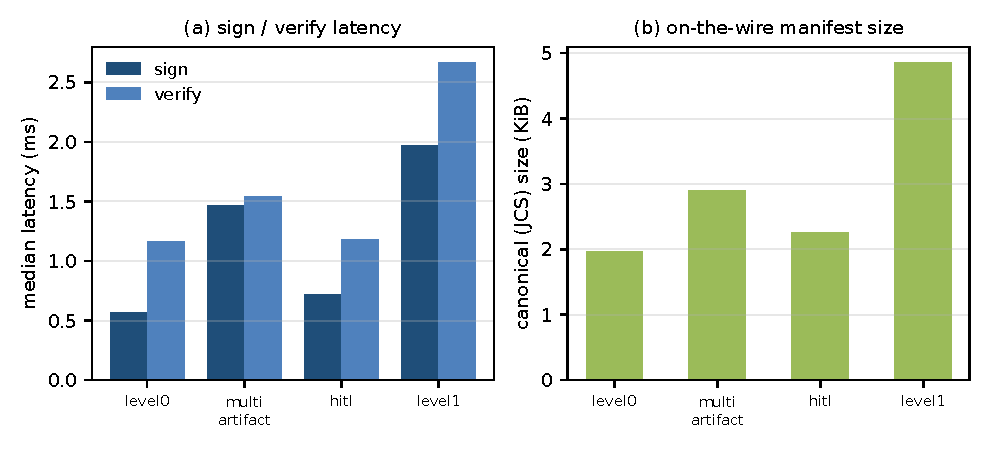
\includegraphics[width=\linewidth]{figures/sign_verify_size.pdf}
\caption{(a) Median Ed25519 sign and verify latency and (b) canonical (JCS) manifest
size across the committed example manifests. Generated by \texttt{experiments/plot.py}
from the measured \texttt{bench.json}.}
\label{fig:signsize}
\end{figure}

\paragraph{Delegation-chain scaling.}
We built signed delegation chains of depth 1 to 10 using the shipped
\texttt{DelegationHopSigner}, narrowing scope monotonically at each hop (dropping one
tool and decrementing the depth budget), and verified each chain with the shipped
\texttt{verify\_delegation\_chain}. Verification latency is close to linear in
chain depth (Figure~\ref{fig:deleg}): depths 1 to 9 cost about 0.21\,ms per hop
(0.21\,ms for one hop, 1.99\,ms for nine), and the ten-hop median, 2.96\,ms, sits
above that line.

\begin{figure}[h]
\centering
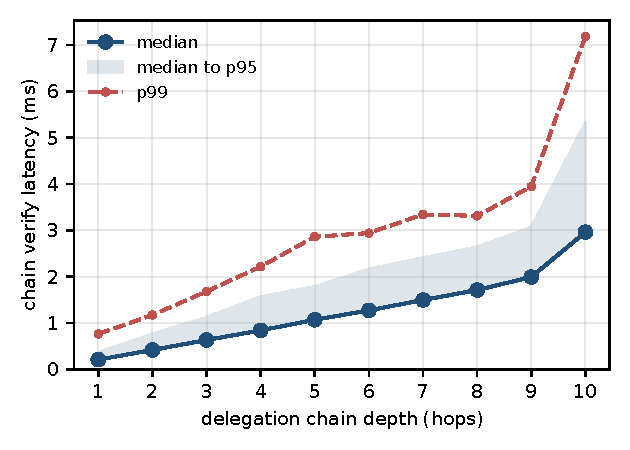
\includegraphics[width=0.62\linewidth]{figures/delegation_latency.pdf}
\caption{Delegation-chain verification latency versus chain depth (1 to 10 hops),
median with the median-to-p95 band and the p99 line. Each hop is signed by the shipped
\texttt{DelegationHopSigner} and verified by \texttt{verify\_delegation\_chain}.}
\label{fig:deleg}
\end{figure}

\paragraph{Tamper detection.}
Starting from a signed Level~1 manifest that verifies \texttt{VALID}, we mutated each
of ten bound fields in turn (six artifact fields, namely five digests and the model
version, plus \texttt{agent\_id}, \texttt{issuer}, \texttt{manifest\_id}, and
\texttt{issued\_at}) and re-verified without re-signing. In all ten cases
verification no longer returned \texttt{VALID}: the mutated canonical bytes fail the
single signature, so the tamper is caught (fail-closed). This shows that the
signature covers these fields. The probe supplies no runtime artifact digests, so
comparison against a deployed agent's artifacts is not exercised. The verifier at
this revision also did not recompute the declared tool-catalog root from the per-tool
entries: the committed Level~0 example declares a root that its own tool list does
not produce, verifies \texttt{VALID} here, and returns \texttt{MISMATCH} on current
SDK main.
